%!TEX root = ../../main.tex

\chapter{Buttons}
\label{cha:buttons}

For the following sections there exist a shared component called \androidinline{GirafButton} which assists one to comply with the following design rules, for a guide on how to use this class see \appref{app:usage_of_girafbuttons}.

\section{States}
\label{sec:button_states}

A button should contain three sates: default, pressed and disabled. The background of a default button should have a orange/yellow (\colref{2.1}) gradient background with a darker border (\colref{2.2}) as seen in \figref{fig:girafbutton_default}. When a button is pressed the background should become darker (\colref{2.3}) alongside the an even darker border (\colref{2.4}) as seen in \figref{fig:girafbutton_pressed}. When a button is disabled the background and the border should be identical to the default button however this button should be 65\% opaque \figref{fig:girafbutton_disabled}.

\begin{figure}[!htbp]
    \centering

    \begin{subfigure}[t]{0.3\textwidth}
    	\centering
        
\includegraphics[scale=0.18]{girafbutton_default}
        \caption{Default}
        \label{fig:girafbutton_default}
    \end{subfigure}
    \hspace{1em} 
    \begin{subfigure}[t]{0.3\textwidth}
    	\centering
        
\includegraphics[scale=0.18]{girafbutton_pressed}
        \caption{Pressed}
        \label{fig:girafbutton_pressed}
    \end{subfigure}
    \hspace{1em} 
    \begin{subfigure}[t]{0.3\textwidth}
    	\centering
        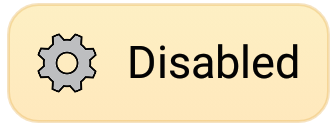
\includegraphics[scale=0.18]{girafbutton_disabled}
        \caption{Disabled}
        \label{fig:girafbutton_disabled}
    \end{subfigure}
    
    \caption{Sates of a button}
    \label{fig:girafbutton_states}
\end{figure}

\section{Content}
\label{sec:button_content}

A button can either contain text (\figref{fig:girafbutton_text}), and icon (\figref{fig:girafbutton_icon}) or both as seen in (\figref{fig:girafbutton_both}). If one wants a button that does something that can be symbolized easily with an icon (See \charef{cha:icons}) which the user is familiar with, one should use an icon only button. In other cases where some text is needed to explain an action one should do so, how ever one should only have both icon and text in cases where the icon helps to understand the text. In the cases where there are no icon symbolizing what the text describes one should use a text only button.

\begin{figure}[!htbp]
    \centering

    \begin{subfigure}[t]{0.3\textwidth}
    	\centering
        
\includegraphics[scale=0.18]{girafbutton_text}
        \caption{Button with text}
        \label{fig:girafbutton_text}
    \end{subfigure}
    \hspace{1em} 
    \begin{subfigure}[t]{0.3\textwidth}
    	\centering
        
\includegraphics[scale=0.18]{girafbutton_icon}
        \caption{Button with icon}
        \label{fig:girafbutton_icon}
    \end{subfigure}
    \hspace{1em} 
    \begin{subfigure}[t]{0.3\textwidth}
    	\centering
        
\includegraphics[scale=0.18]{girafbutton_both}
        \caption{Button with both}
        \label{fig:girafbutton_both}
    \end{subfigure}
    
    \caption{Content of a button}
    \label{fig:girafbutton_content}
\end{figure}

\section{Context}
\label{sec:button_context}

When a collection of buttons is shown regarding the same context the buttons should be ordered by negative and positive actions. Leftmost buttons should cause negative actions and the rightmost should cause positive buttons. An example of this can be seen in the dialog displayed in \figrefpage{fig:profiles_selector_dialog}.